\section{Zero income events}\label{zero_inc}

Until now, the version of the model examined saw agents save purely due to the no-borrowing constraint, as opposed to a need to save due to any form of uncertainty. As long as agents did not borrow, they were guaranteed positive wealth in the next period due to the next period's income. In this section, in the style of \citet{Carroll1997}, I relax the no-borrowing constraint, and instead introduce a zero-income event that induces the precautionary saving motive. Let the income process now be modelled as
\begin{align*}
    P_{t} &= \G_{t}\eta_{t}P_{t-1}\\
    Y_{t} &= P_{t}\psi_{t}
\end{align*}
where $\psi_{t}$ is modelled as
\[
\psi_{t} = \begin{cases}
    0 & \text{with probability } \xi\\
    \z_{t} & \text{with probability } (1-\xi)
\end{cases}
\]
and the realization of the zero-income event is independent of the realization of the any of the other three shocks. The normalized intertemporal budget constraint can then be rewritten as
\[
m_{t} = \frac{\Rc_{t}}{\Gc_{t}}(m_{t-1} - c_{t-1}) + \psi_{t}
\]
Where the introduction of $\psi_t$ makes the only difference. The joint distribution of $(\eta,\,\nu,\,\z)$ remains unchanged. In the finite-horizon version of the model, consumers may face zero-income events till period $T$, which means that no-default condition at the end of life is enough to ensure that consumers do not borrow. On the other hand, we can introduce a standard no-Ponzi condition in the infinite horizon version of the model to the same effect. As such, I numerically solve for the optimal policy functions only over a domain of positive savings.

One of the possible contentions with modelling the zero-income event as independent of asset return shocks could be that recessions are periods of layoffs, and therefore increasing unemployment. It would then be natural for the probability of the zero-income event to be greater conditional on lower returns on equity. While this is a valid line of reasoning, it is currently beyond the scope of this paper to introduce this added layer of complexity. Another interpretation that can be accorded to zero-income events are major unforeseen expenditures such as on healthcare, which can be approximated as situations where the consumer's net disposable income to spend on the consumption good is near zero. In such situations, they must consume using their savings.

\subsection{Results}

Following the same parameterization as in the previous section, with the added parameter $\xi$ set at 0.005 (see Table \ref{tab:model_parameters}), we can compute the optimal portfolio allocation rule for various settings of $\o_{\eta,\,\nu}$. These can be seen in Figure \ref{fig:zeroInc_shareLimit}.

\begin{figure}[h]
    \centering
    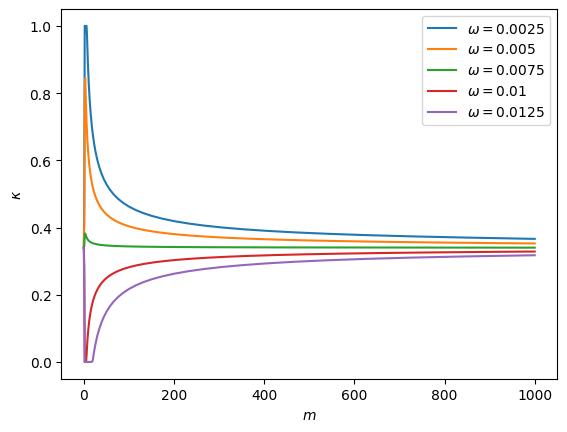
\includegraphics[width=0.6\textwidth]{ShareLimit_permInc_zeroInc.png}
    \caption{Optimal portfolio allocation with zero-income events and income growth and asset return covariance}
    \label{fig:zeroInc_shareLimit}
\end{figure}

Like in the case with the no-borrowing constraint, as the correlation between the income growth and asset return shocks increases, low and moderate wealth individuals begin investing a greater proportion of their wealth in the safe asset. A departure, however, is that irrespective of the correlation, individuals well below the target wealth level choose to invest a shade above 30 percent of their wealth in equity. This, of course, does not reconcile with real-world observations, where the extremely poor often do not enter the equity market. On the other hand, like in the model with the no-borrowing constraint, the limiting value of the optimal portfolio allocation as $m \to \infty$ is largely unaffected by the correlation parameter.

A closer looks reveals that the equity portfolio share tends to the Merton-Samuelson limit as $m \to 0$ as well. This is because as $m$ goes to 0, the marginal utility of consumption conditional on the realization of the zero income event grows arbitrarily large. As such, the weight placed on a realization such that the ratio of labor income to wealth is 0 grows arbitrarily large when solving the optimization problem implied by the excess return equation. This causes the portfolio share of equity to tend to the optimal share in the model without income.

\begin{figure}[h]
    \centering
    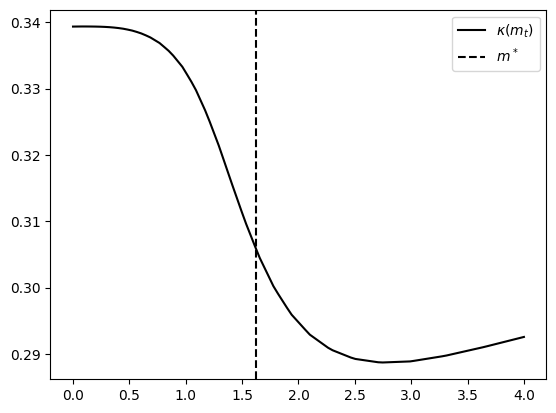
\includegraphics[width=0.6\textwidth]{kFunc_zeroInc_target.png}
    \caption{Optimal portfolio allocation at target wealth with zero-income events}
    \label{fig:zeroInc_target}
\end{figure}

Figure \ref{fig:zeroInc_target} shows the most significant way in which the zero-income event affects the distribution. As opposed to the case with the no-borrowing constraint, consumers would want to hold some of their savings in equity at the target level of wealth, which means that a distribution of agents facing idiosyncratic shocks would also be centered around a reasonable portfolio share. However, an issue one would be hard-pressed to reconcile with the data is that the equity portfolio share is actually decreasing in wealth around the target level, which makes for a counterintuitive prediction.

\subsection{Calibrating to U.S. Data}\label{us_data}

While the previous sections distill the primary insights from the model with an artificial parameterization of asset returns, both in terms of the equity premium and the variability of the returns from equity, I now look at how the model responds to being calibrated to parameters documented in the literature about U.S. data. Since the primary determinant of optimal portfolio allocation in the model that is of interest to us is the correlation between permanent income shocks and shocks to the return on the risky asset, I vary this parameter while holding the others constant at documented values. To begin, \citet{Mehra1985} estimate that the historical real rate of return on equity in the U.S. is 7.67 percent, while the return on a relatively risk-free securities over the same period was 1.31 percent.\footnote{The original data was later updated till 2005, which forms the source of these estimates. See \citet{Mehra2006} for details.} Furthermore, the Sharpe ratio for these assets was calculated to be 0.37. Since $\nu$ is a mean-one lognormal, we know that:
\[
\s_{\nu}^2 = \log\bp{\bp{\frac{\Rfree - \Rfix}{0.37\Rfree}}^2 + 1}
\]
I follow \citet{Carroll1992} and set the standard deviations of logged permanent and transitory income shocks to 10 percent. Following the same paper, I set permanent income growth at 3 percent and the probability of the zero income event as 0.5 percent. I also set $\b = 0.93$ and $\o_{\z,\,\eta} = \o_{\z,\,\nu} = 0$. I then solve the model using a baseline of $\rho = 4$ for different values of $\o_{\eta,\,\nu}$. The full choice of parameters is then given in Table \ref{tab:model_parameters}.

\begin{table}[htbp]
    \begin{tabular}{ccc}
        \toprule
        Parameter & Value & Source\\
        \midrule
        $\rho$ & 4\\
        $\b$ & 0.93\\
        $\G$ & 1.03 & \citet{Carroll1992}\\
        $\Rfree$ & 1.0767 & \citet{Mehra2006}\\
        $\Rfix$ & 1.0131 & \citet{Mehra2006}\\
        $\s_{\nu}^2$ & 0.011 & \citet{Mehra2006}\\
        $\s_{\eta}^2$ & 0.01 & \citet{Carroll1992}\\
        $\s_{\z}^2$ & 0.01 & \citet{Carroll1992}\\
        $\xi$ & 0.005 & \citet{Carroll1992}\\
        \bottomrule
    \end{tabular}
    \caption{Parameters used to solve the model}
    \label{tab:model_parameters}
\end{table}

The first thing we can see under this new parameterization is that even with highly collinear shocks ($\text{corr}(\log\nu,\,\log\eta) \approx 1$), the optimal portfolio share is 1. This is because despite the high covariance, the excess return of more than 6 percent and the relatively low volatility, with a standard deviation of under 10.5 percent for the logged shock to returns, makes it difficult to justify holding the risk-free asset. In fact, Figure \ref{fig:US_rho_comparison} shows that the equity share of portfolio falls to realistic levels under the no-borrowing constraint only when $\rho$ is as large as 12. This number is close to the benchmark by \citet{Schreindorfer2020}, whose model incorporates disappointment averse preferences and has agents exhibit levels of relative risk aversion of close to 10.

\begin{figure}[h]
    \centering
    \begin{subfigure}{0.49\textwidth}
        \centering
        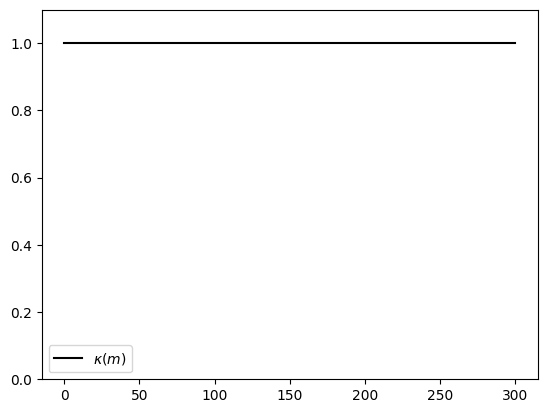
\includegraphics[width=0.8\textwidth]{kFunc_US_rho4.png}
        \caption{$\rho = 4$}
    \end{subfigure}
    \begin{subfigure}{0.49\textwidth}
        \centering
        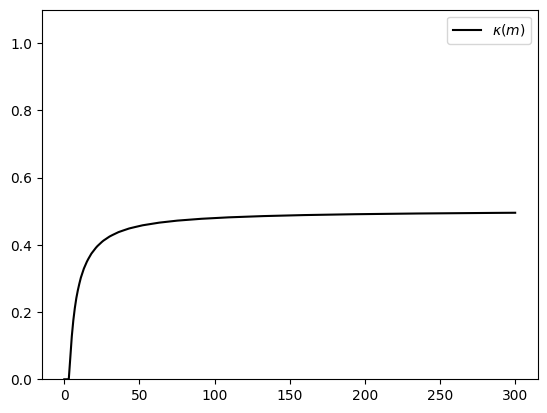
\includegraphics[width=0.8\textwidth]{kFunc_US_rho12.png}
        \caption{$\rho = 12$}
    \end{subfigure}
    \caption{U.S. figures requires extremely high RRA to explain the equity premium}
    \label{fig:US_rho_comparison}
\end{figure}

The limiting value of the portfolio share of equity is not very different under the model with zero-income events. In fact, the limiting portfolio share of equity is identical between the two models. What changes is how we can explain the equity share around the target wealth.

\begin{figure}[h]
    \centering
    \begin{subfigure}{0.49\textwidth}
        \centering
        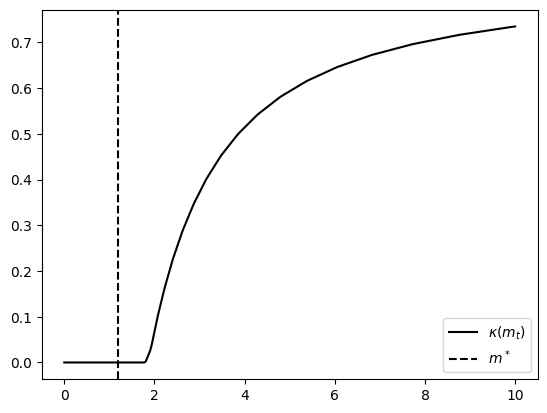
\includegraphics[width=0.9\textwidth]{kFunc_US_target.png}
        \caption{$\rho = 7$, NBC}
    \end{subfigure}
    \begin{subfigure}{0.49\textwidth}
        \centering
        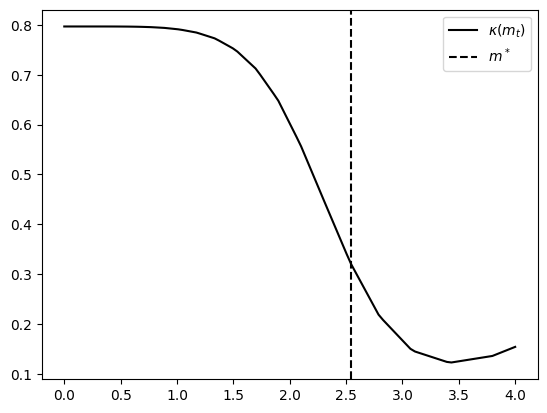
\includegraphics[width=0.9\textwidth]{kFunc_US_zeroInc.png}
        \caption{$\rho = 7.5$, Zero Income Events}
    \end{subfigure}
    \caption{Portfolio share around target wealth under the no-borrowing constraint and zero-income events}
    \label{fig:US_zeroInc_target}
\end{figure}

Figure \ref{fig:US_zeroInc_target} shows that for $\rho = 7.5$, optimal portfolio share around the target wealth actually falls to around 30\%. Meanwhile, in the model with the no-borrowing constraint, the equity share at target is 0. This is so, even as the limiting values of share holdings under this parameterization are really high. As such, while the model with zero income events makes for a better approximation around the target wealth, it performs identically to the model with the borrowing constraint for high $m_t$ and worse by predicting that the poor will invest close to the share limit in equity, particularly as $m_t \to 0$. In any case, a value for $\rho$ greater than 7 does not produce suitable implications for consumption-savings behavior.

These findings show that while these models do not explain the equity premium perfectly, the introduction of the correlation between permanent income shocks and asset returns has produced a significant improvement in how optimal portfolio decisions fit the data at relatively reasonable levels of risk aversion. Furthermore, while the model with the no-borrowing constraint accurately prohibits the extremely poor from investing in equity, the introduction of the zero income events ensures that consumers engage in precautionary saving and invest some of their fairly substantial savings in equity as a result.